\documentclass[mathserif,utf8,xcolor=table,10pt]{beamer}

\usepackage[T2A]{fontenc}
\usepackage[utf8]{inputenc}
\usepackage[english,russian]{babel}
\usepackage{graphicx}
\usepackage{ulem}
\usepackage{textpos}
\usepackage{hyperref}
%\usepackage{listings}
\usepackage{listingsutf8}
%\usepackage{minted}
\usepackage{tikz}
\usetikzlibrary{mindmap,shadows}
%\usepackage[hidelinks,pdfencoding=auto]{hyperref}


\definecolor{dkgreen}{rgb}{0,0.6,0}
\definecolor{gray}{rgb}{0.5,0.5,0.5}
\definecolor{mauve}{rgb}{0.58,0,0.82}

\lstset{frame=single,framerule=0pt,
  language=C++,
%  aboveskip=3mm,
%  belowskip=3mm,
  showstringspaces=false,
  columns=flexible,
  basicstyle={\scriptsize\ttfamily},
  numbers=none,
  numberstyle=\tiny\color{gray},
  keywordstyle=\color{blue},
  commentstyle=\color{dkgreen},
  stringstyle=\color{mauve},
  breaklines=true,
%  breakatwhitespace=true,
  tabsize=2,
 % escapeinside={\%*}{*)},
 % inputencoding=utf8,
  inputencoding=utf8/utf8,
  texcl=true,
}

\mode<presentation>
{
        \usetheme{Antibes}
        \setbeamercovered{transparent}
}

\title{Объектно-ориентированное программирование (ООП, OOP): принципы, классы, объекты, прототипы}
\institute{Степулёнок Денис Олегович}
\date[январь 2016]{13 января 2016 года}
\subject{Занятие 4}

\newcommand{\hl}{\only{\cellcolor{yellow}}}
\renewcommand{\le}{\leqslant}
\renewcommand{\ge}{\geqslant}
\setlength{\arrayrulewidth}{1pt}

\begin{document}

% ООП в C++. Часть 1

\section{ООП - принципы: классы, объекты, прототипы} 

\subsection{Абстракция, класс, объект, прототип}

\begin{frame}[t,fragile]{Объектно-ориентированное программирование}

Способ программирования, в котором используются 
\textbf{объекты}
 и 
\textbf{классы}. 

\textbf{Абстрагирование} --- 
выделение набора важных с точки зрения решаемой задачи характеристик объекта, исключая из рассмотрения неважные. 

\textbf{Абстракция} --- 
набор всех важных характеристик объекта, реализуется в ООП-языках при помощи Класса. 

Пример: решаем задачу с точками на плоскости, для каждой
точки важны её координаты $(x; y)$.

\textbf{Класс} ---
создаваемый программистом новый тип данных,
модель ещё не существующей сущности (объекта).

\begin{lstlisting}
class Point { double x,y; }
\end{lstlisting}

\textbf{Объект} --- 
конкретная <<точка>>, экземпляр класса.

\begin{lstlisting}
Point A = {2.0, 1.5}, B = {-2, 1};
\end{lstlisting}

\textbf{Прототип} ---
объект-образец, по образу и подобию которого создаются другие объекты
путём копирования и изменения различных свойств. 
\end{frame}

\subsection{Инкапсуляция, наследование и полиморфизм}

\begin{frame}[t]{Принципы ООП}

\textbf{Инкапсуляция} --- свойство системы, позволяющее объединить данные и методы, 
работающие с ними, в классе, и скрыть детали реализации от пользователя.

\textbf{Наследование} --- свойство системы, позволяющее описать новый класс на основе 
уже существующего с частично или полностью заимствующейся функциональностью. 
Класс, от которого производится наследование, называется 
\textbf{базовым}, \textbf{родительским} или \textbf{суперклассом}. 
Новый класс --- \textbf{потомком}, \textbf{наследником}, \textbf{дочерним} или \textbf{производным} классом.

\textbf{Полиморфизм} --- свойство системы использовать объекты с одинаковым интерфейсом без информации о типе и внутренней структуре объекта.
При использовании термина <<полиморфизм>> в сообществе ООП подразумевается полиморфизм подтипов; 
а использование параметрического полиморфизма называют обобщённым программированием.

\end{frame}
                     
\subsection{Объявление класса: аттрибуты, поля, методы}
\begin{frame}[t,fragile]{Класс <<Точка>> --- не используя ООП}

Если нам нужно хранить 100 точек, то мы можем создать 2 независимых массива:
\begin{lstlisting}
double x[100], y[100];
\end{lstlisting}

И синхронно их использовать:
\begin{lstlisting}
  x[0] = 1;  y[0] = 2;
\end{lstlisting}

Или создать структуру точка:
\begin{lstlisting}
struct Point {
  double x, y;
};
\end{lstlisting}

Чтобы потом создать массив из точек:
\begin{lstlisting}
Point p[100];
\end{lstlisting}

И обращаться к нему:
\begin{lstlisting}
  p[0].x = 1; p[0].y = 2;
  Point p1; p1.x = 2;
\end{lstlisting}
\end{frame}

\subsection{Объявление и использование класса}
\begin{frame}[t,fragile]{Объявление и использование класса}

Объявление класса <<Point2D>>:
\begin{lstlisting}
class Point2D {
 public:
  double x, y; // Поля (данные) класса
  // Метод класса <<Передвинуть точку>>
  void move(double dx, double dy) { x += dx; y += dy; }
  // Повернуть точку относительно начала координат
  void rotate(double angle) { ... }
};
\end{lstlisting}

Использование класса:
\begin{lstlisting}
  Point2D p[100]; // Массив
  p[10].x = 10.1;  p[10].y = 10.3;
  p[0].move(1, 2);
\end{lstlisting}

\end{frame}

\subsection{Более сложный пример - стек}

\begin{frame}[t,fragile]{Более сложный пример - стек}
\begin{lstlisting}
// Объявление класса
class Stack { // класс ИмяКласса
  // Константы
  const static int STACK_SIZE = 100; // Размер стека
  // private-поля класса
  int data[STACK_SIZE]; // Данные
  int count = 0; // Сколько элементов в стеке сейчас
 public: // public-методы - те, операции которые будем использовать извне
  // Положить данные на вершину стека
  void push(int value) { // тип\_возвр\_значения имя \(аргументы\)
    if(count == STACK_SIZE) { // Стек полон
      cout << "Stack is full!" << endl;
      return;
    }
    data[count++] = value; // Записываем значение и увеличиваем количество
  }
  // Забрать данные с вершины стека
  int pop() {
    if(count == 0) { // Стек пуст
      cout << "Stack is empty!" << endl;
      return -1; // Не можем ничего не вернуть
    }
    return data[--count]; // Уменьшаем количество и возвращаем значение
  }
};
\end{lstlisting}
\end{frame}

\begin{frame}[t,fragile]{Более сложный пример - стек - пример использования}
\begin{lstlisting}
int main(){
  Stack s; // Создание переменной - экземпляра стека
    // Стек пуст
  s.push(2); // Положим в стек число 2
    // Теперь стек: | 2 |
  s.push(3); // а затем число 3
    // Теперь стек: | 3 | 2 |
  cout << "3 - " << s.pop() << endl; // Должно быть 3
    // Теперь стек: | 2 |  
  cout << "2 - " << s.pop() << endl; // Должно быть 2
    // Извлекли все значения - снова пуст 
  return 0;
}
\end{lstlisting}
\end{frame}

 
% * Создание экземпляра 
\subsection{Конструкторы и деструкторы}

\begin{frame}[t,fragile]{Конструкторы и деструкторы}

\textbf{Конструктор} (construct - создавать) --- 
специальный метод класса, который выполняется после создания объекта и предназначен для инициализации 
полей класса некоторыми начальными значениями.

Несколько конструкторов должны отличаться типами передаваемых значений.

\textbf{Деструктор} (destruct - разрушать) --- 
специальный метод класса, который служит для уничтожения 
элементов класса и выполняется перед удалением объекта. 

В классе может быть только один деструктор.

\end{frame}

\subsection{Конструкторы и деструкторы - MyClass}

\begin{frame}[t,fragile]{Конструкторы и деструкторы - пример}
\begin{lstlisting}
class MyClass {
  static int count; // Количество объектов
  int id; // Идентификатор данного объекта
  int* data;
  char* name;
 public:
  // Конструктор - после создания экземпляра (объекта) класса
  MyClass(char*);
  // Деструктор - перед уничтожением экземпляра (объекта)
  ~MyClass();
};
// Инициализация static-переменной
int MyClass::count = 0;

MyClass::MyClass(char* n = "") : name(n), id(++count) {
  cout << "Constructor #" << id << " " << name << endl;
  data = new int[1000]; // Отводим динамическую память
  data[0] = 10; // Используем её как хотим
}
MyClass::~MyClass() {
  cout << "Destructor #" << id << " " << name << endl;
  delete[] data; // Освобождаем динамическую память
}
\end{lstlisting}
\end{frame}



% * Конструкторы и деструкторы классов. Возможности инициализации объектов. Копирующий конструктор.
% * Определение и перегрузка операторов класса в C++. Вывод в поток.
% * Прототипы
% * Практика: класс "рациональная дробь"



% 2. Организация совместной работы, системы контроля версий
% * Системы контроля версий: централизованные, распределённые
% * История версий, ветки
% * Основы работы с git
\section{Системы контроля версий}
\subsection{Что такое контроль версий, и зачем он вам нужен?}

\begin{frame}[t]{Что такое контроль версий, и зачем он вам нужен?}

Система контроля версий (СКВ) — это система, регистрирующая изменения в одном или нескольких файлах с тем, 
чтобы в дальнейшем была возможность вернуться к определённым старым версиям этих файлов. 

СКВ даёт возможность возвращать отдельные файлы к прежнему виду, 
возвращать к прежнему состоянию весь проект, 
просматривать происходящие со временем изменения, определять, 
кто последним вносил изменения во внезапно переставший работать модуль, 
кто и когда внёс в код какую-то ошибку, и многое другое. 
Вообще, если, пользуясь СКВ, вы всё испортите или потеряете файлы, всё можно будет легко восстановить. 

Системы контроля версий:
\begin{itemize}
  \item Централизованные 
  \item Децентрализованные
\end{itemize}

\end{frame}

\subsection{Системы контроля версий: локальные, централизованные, распределённые}

\begin{frame}[t]{Subversion}

Бесплатная система управления версиями с открытым исходным кодом.
Subversion позволяет управлять файлами и каталогами, а так же сделанными в них изменениями
во времени. Это позволяет восстановить более ранние версии данных, даѐт возможность изучить
историю всех изменений. Благодаря этому многие считают систему управления версиями своего
рода «машиной времени».

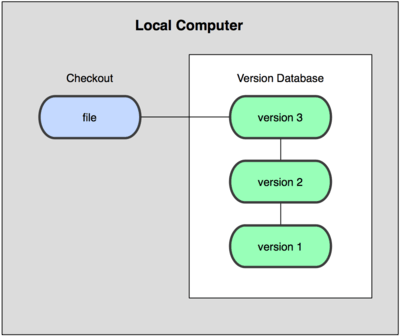
\includegraphics[width=0.5\textwidth]{git/rcs.png}

\end{frame}

\begin{frame}[t]{Централизованные системы контроля версий}
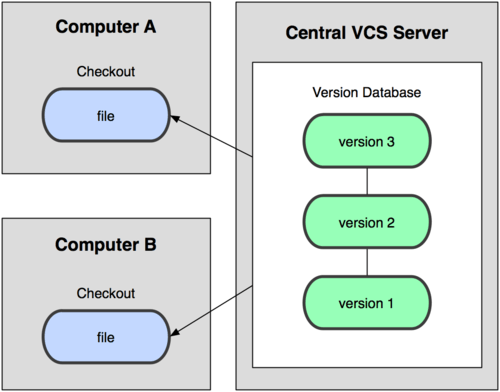
\includegraphics[width=0.5\textwidth]{git/central.png}
\end{frame}

\begin{frame}[t]{Распределённые системы контроля версий}
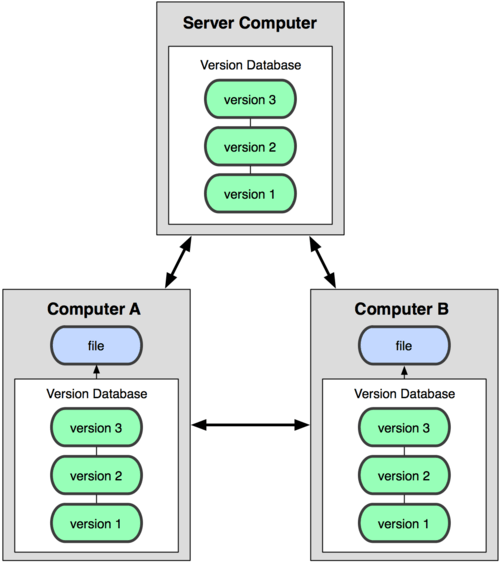
\includegraphics[width=0.5\textwidth]{git/distrib.png}
\end{frame}

\begin{frame}[t]{Git}

Распределённая система управления версиями. 
Проект был создан Линусом Торвальдсом для управления разработкой ядра Linux, первая версия выпущена 7 апреля 2005 года. 
На сегодняшний день его поддерживает Джунио Хамано.

Примерами проектов, использующих Git, являются:
ядро Linux, Android, Drupal, Cairo, GNU Core Utilities, Mesa, Wine, Chromium, Compiz Fusion, FlightGear, jQuery, PHP, NASM, MediaWiki, DokuWiki, Qt и некоторые дистрибутивы Linux 

\url{}

\end{frame}

\begin{frame}[t]{Откуда скачать и установить Git?}


Для Windows --- \url{https://git-for-windows.github.io}

Нажимаете \textbf{Download}, скачивается исполняемый файл, например 
\textbf{Git-2.6.1-64-bit.exe}

Устанавливаете его. 

После установки должна появится в командной строке команда:
\texttt{git}

\end{frame}

 
\subsection{История версий, ветки}
\begin{frame}[t]{Основные команды Git}

\texttt{git init} --- создание нового git-репозитория в текущей папке.
С этого момента в этой папке появляется <<машина времени>> для изменений.
Если вы сделали изменение и зафиксировали его, вы всегда можете откатиться к этой версии.

При успешной инициализации выводится сообщение:
Initialized empty Git repository in FolderName

\texttt{git add} --- добавление файлов в систему контроля версий.
Например: \texttt{git add a.cpp} --- добавить файл a.cpp в СКВ.
\texttt{git add *.cpp} --- добавить все .cpp файлы в СКВ. 
\texttt{git add .} --- добавить все файлы и все каталоги с подкаталогами в СКВ. 

\end{frame}

\subsection{Почитать про Git}
\begin{frame}[t]{Основные команды Git}

\end{frame}
                                         



% * Виды тестирования и отладки
%\section{Тестирование и отладка}

\subsection{Методы тестирования и отладки}

\begin{frame}[t]{Методы тестирования и отладки}

  \begin{itemize}
    \item Ручное тестирование / ручная отладка --- Steps to reproduce / шаги "как воспроизвести" - 
      недостаток - слишком много ресурсов на повторение шагов каждый раз
    \item Использование отладчика (debugger)
    \item Логгирование (протоколирование) --- Единственный, который доступен на компьютере конечного пользователя
    \item Автоматические тесты
    \begin{itemize}
      \item Модульные: Unit-тесты
      \item Функциональные:
      \begin{itemize}
        \item По спецификации 
        \item Регрессионные тесты
      \end{itemize}
      \item Интеграционные тесты (integration)
      \item Тесты производительности (perfomance)
    \end{itemize}  
  \end{itemize}
\end{frame}


% Приоритет операций
%\section{Приоритет операций в C/C++}

\subsection{Приоритет операций}

\begin{frame}[t,fragile]{Арифметические операции}

\begin{lstlisting}
  double x = 10 / 2 * 5;
  cout << "x = " << x << endl; // 25
  double x2 = 10 / (2 * 5);
  cout << "x2 = " << x2 << endl; // 1
  cout << 10.0 / 2.0 / 5.0 << endl; // 1.0
\end{lstlisting}

Всегда ставьте скобки, если не очевиден порядок.
 
\end{frame}


% Чтение и запись текстовых файлов 
\section{Типы данных С++}
\subsection{Целочисленные типы данных}

\begin{frame}[t]{Целочисленные типы данных}
  1 байт:
  \begin{itemize}
    \item \texttt{bool} --- логический тип данных: \texttt{true} / \texttt{false}
    \item \texttt{char} --- символьный тип данных от $-128$ до $127$ или $0..255$ \texttt{unsigned char}
  \end{itemize}
  2 байта:
  \begin{itemize}
    \item \texttt{short int}, \texttt{short} --- от $-2^{15}=-32.768$ до $2^{15}-1=32.767$
    \item \texttt{unsigned short int} --- от $0$ до $2^{16}-1=65.535$
  \end{itemize}
  4 байта:
  \begin{itemize}
    \item \texttt{int}, \texttt{long int}, \texttt{long}, \texttt{signed} --- от $-2^{31}=-2.147.483.648$ до $2^{31}-1=2.147.483.647$
    \item \texttt{unsigned int}, \texttt{unsigned long int}, \texttt{unsigned long}, \texttt{unsigned} --- от $0$ до $2^{32}-1=4.294.967.295$
  \end{itemize}
  8 байт:
  \begin{itemize}
    \item \texttt{long long, \_\_int64} --- от $-2^{63}=-9.223.372.036.854.775.808$ до $2^{63}-1=9.223.372.036.854.775.807$
    \item \texttt{unsigned long long, unsigned \_\_int64} --- от $0$ до $2^{64}-1=18.446.744.073.709.551.615$
  \end{itemize}
\end{frame}




% * Литература по C/C++.

\end{document}
